\documentclass[a4paper, 12pt]{report}

\usepackage[utf8]{inputenc} %pour avoir les accents
\usepackage[T1]{fontenc} %pour gerer où couper les mots et les accents dans le pdf
\usepackage[francais]{babel} % pour avoir la typo francaise
\usepackage[a4paper]{geometry} % s'adapte à une feuille a4
\usepackage{setspace} % gere les espaces entre les lignes
\usepackage{color} %gere les couleurs
\usepackage{listings} % pour avoir des lignes de codes
\usepackage{hyperref} % gere les url
\usepackage{amssymb}  %pour les formules de math
\usepackage{graphicx} % pour gerer les images
%\usepackage[nottoc]{tocbibind} % gere la bibliographie

\begin{document}

%%%%%%%%%%%%%%%%%%%%%%%%%%%%% Page de garde
\begin{titlepage}

%%%%%% Entête
\begin{figure}[t]
\begin{center}

\includegraphics[width=0.45\textwidth]{ub.png}

\includegraphics[width=0.45\textwidth]{scrime.png}
\end{center}
\vspace{1cm}
\end{figure}

\begin{center}
{\LARGE Licence d'Informatique\\Rapport de Stage\\Du 5 novembre 2015 au 27 juin 2016\\}
\end{center}
%%%%%% Fin Entête

%%%%%% Titre
\begin{center}
\vspace{1.4cm}
\fbox{
	\begin{minipage}{\textwidth}
	\begin{center}
	{\color{cyan} \Huge Interface de pilotage \\du robot "Thymio" avec I-score\\}
	\end{center}
	\end{minipage}
	}
\end{center}
%%%%%% Fin Titre	
\vspace{1.4cm}

%%%%%% Personnes
\begin{description}
\item[{\LARGE Stagiaire:}{ Gaëtan CHAMBRES}]
\item[{\LARGE Responsable de stage:}{ Pierre COCHARD}]
\vspace{0.5cm}
\item[{\LARGE Co-dirigeant de stage:}{ Phillipe GUILLEM}]
\end{description}

%%%%%% Fin Personnes
\vspace{1.4cm}
%%%%%% Adresse
\begin{description}
\item[Stage effectué au sein de:]
\item[Université de Bordeaux]
\item[351 cours de la libération]
\item[33405 Talence cedex]
\end{description}

%%%%%% Fin Adresse


\end{titlepage}
%%%%%% fin de la page de garde


\chapter*{Remerciements}
\pagenumbering{roman}

%%%%%%%%%

A RÉDIGER PLUS TARD

%%%%%%%%%%

\chapter*{Résumé}

%%%%%%%%%

A RÉDIGER PLUS TARD

%%%%%%%%%%


\tableofcontents %génére la table des matieres

\chapter{Introduction}
\pagenumbering{arabic} % reinitialise le compteur et numerote les pages en chiffres arabes
\section{Domaine du Stage}
\subsection{Le SCRIME \cite{scrime2015}}
Ce stage a été effectué au sein du Studio de Création et de Recherche en Informatique et Musiques Expérimentales( ou Électro-acoustiques).\\
Ce groupement d'intérêt scientifique et artistique est rattaché à l'équipe Image et Son du Laboratoire Bordelais de Recherche en Informatique (LaBRI).\\
Les champs d'activités du SCRIME s'étendent de la recherche scientifique à la création artistique, en passant par la formation, la diffusion des musiques contemporaines et la pédagogie en milieu scolaire et universitaire. \\
Le SCRIME est soutenu par le Ministère de la Culture, le Conseil Régional d'Aquitaine, la DRAC et le CNRS.\\

\subsection{Les missions du SCRIME \cite{scrime2015}}
Les différentes missions du SCRIME sont:
\begin{itemize}
\item Favoriser la collaboration entre scientifiques et artistes à des fins de recherche et de création
\item Favoriser la diffusion internationale des résultats des recherches et des oeuvres artistiques
\item Promouvoir les collaborations scientifiques et artistiques avec d'autres centres de recherche et de création en France ou à l'étranger
\item Favoriser les actions pédagogiques dans les institutions partenaires ainsi que dans les autres établissements publics d'enseignement et de création et ce à tous les niveaux 
\end{itemize}

\subsection{L'équipe du SCRIME \cite{scrime2015}}
L'équipe de ce groupement d'intérêt scientifique et artistique est essentiellement composée de:
\begin{description}
\item[Myriam Desainte-Catherine :] Direction scientifique
\item[Jean-Louis Agobet :] Direction artistique
\item[Gyorgy Kurtag :] Coordination Arts et Sciences
\item[Annick Mersier :] Gestionnaire
\item[Christian Faurens :] Assistant ingénieur audiovisuel
\item[Pierre Cochard :] Réalisateur en Informatique Musicale
\item[Antoine Hubineau :] Chargé de communication
\item[Julia Hanadi Al Abed :] Régisseur son
\item[Jean-Michel Rivet :] Compositeur et Enseignant
\item[Raphaël Marczak :] Ingénieur de recherche
\item[Nicolas Vuaille :] Développeur
\end{description}
Pierre COCHARD  aura été mon responsable de stage, mais j'ai également travaillé avec Philippe GUILLEM, professeur de musique et enseignant en classe de maternelle.

\section{Le contexte du stage}
\subsection{Pourquoi ce projet?}

Philippe GUILLEM est maître formateur en musique et enseignant en école maternelle. Son objectif est de montrer à ses élèves ce que le monde moderne leur offre. Cela va des réseaux sociaux à la robotique, en passant par la programmation de manière plus vaste. Seulement une interrogation naissait en même temps que cette idée :\\

Comment chez des élèves de 5 ans, aider à construire une image du Robot et des relations que l'homme peut entretenir avec ces machines?\\

Lors d'une conférence, Philippe GUILLEM a découvert le projet du robot THYMIO. De part sa robustesse, sa simplicité d'accès, d'utilisation et de programmation, ainsi que par sa conception, il était tout à fait adapté aux jeunes enfants et donc à ce projet.
Enfin, il restait la question de représenter la relation homme / robot. Pour cela, Mr GUILLEM a tenu à faire un lien avec la musique, car c'est ce qu'il y a de plus parlant pour les jeunes auditorats. C'est donc à ce moment que le SCRIME a été sollicité, en particulier Pierre COCHARD, et ils ont travaillé sur le projet de ce stage, qui finira par m'être proposé.


\subsection{Les objectifs du stage}
%%%%%%%%%% TODO MAJ %%%%%%%%%% 
L'objectif principal de ce stage était de réaliser une interface permettant de piloter le robot Thymio avec le logiciel i-score afin d'en permettre l'utilisation en classe avec des élèves de maternelle par monsieur Phillipe GUILLEM. \\
Dans ce but, ce stage devait permettre d'implémentation d'un système de communication entre Pyo (ou tout autre logiciel adapté) et i-score.\\
L'objectif pédagogique était d'obtenir des compétences en robotique et dans le traitement des informations d'un capteur. 

\section{Contenu du rapport}
%%%%%%%%%

%A RÉDIGER PLUS TARD "le résumé" En double??

%%%%%%%%%%
\chapter{Le Robot Thymio}
\section{Présentation \cite{thymio2016}}

Thymio, conçu par l’École polytechnique fédérale de Lausanne est un petit robot dédié à la pédagogie. Ses deux roues lui permettent déplacement et manoeuvres, tandis qu'il embarque des boutons ainsi que de nombreux capteurs infrarouges pour détécter des obstacle ou des surfaces, un micro, un haut parleur, un accéléromètre et même un thermomètre. Son accessibilité est due à la mise à disposition de ses propres interfaces de programmation. Il y en a en effet plusieurs, à commencer par l'interface de programmation texte, ASEBA STUDIO qui permet d'exploiter entièrement le langage ASEBA. Une adaptation de BLOCKY est aussi disponible, qui permet d'aborder la programmation texte de manière simplifiée, et enfin il y a VPL qui permet de programmer THYMIO visuellement grâce à des vignettes. C'est grâce à ces interfaces que ce robot se trouve adpaté aux plus jeunes.

Pour résumer, il s'agit d'un robot complet, qui embarque un grand nombre de capteurs, et accessible à tous, aux plus jeunes comme aux programmeurs confirmés, c'est pourquoi ce robot a été choisi pour ce projet de stage.

\section{Philosophie d'un projet collaboratif\cite{thymio2016}}
Le but du projet THYMIO était de permettre à un large publique, et en particulier aux enfants, la découverte et l'apprentissage de la programmation, de la robotique, de l'ingénierie et des technologies numériques. Pour permettre cela, il a fallut regrouper plusieurs corps de métiers et des connaissances poussées dans différents domaines. C'est pourquoi THYMIO est un projet communautaire, qui implique plusieurs entités. Il s'agit donc d'un modèle basé sur le partage libre des connaissances, c'est à dire que Tout le matériel, le logiciel, et la documentation sont développés par les partenaires sous licence libre. Ainsi, les partenaires s'engagent à fournir l'information de conception gratuitement, de manière à ce que chacun puisse comprendre, utiliser, ou modifier cette information, à condition de distribuer à son tour les résultats de son travail. Il est donc important que ce stage s'inscrive dans cette dynamique, et que le travails ainsi que les résultats soient partagés à la communauté.

\section{Les différents acteurs du projet \cite{thymio2016}}
Comme expliqué précédemment, plusieurs catégories d'acteurs se sont alliés dans ce projet:
\begin{description}
\item[Les institutions de recherche: ]qui permettent de diffuser le travail et de l'amener auprès du public. Plus la base d'utilisateurs grandit, meilleures sont les possibilités d'évaluation et d'amélioration. Les résultats de la recherche sont ainsi mis rapidement en application.
\item[Les entités de production: ] qui donnent accès à des produits proches de l'état de l'art qui n'ont plus qu'à être industrialisés. Les frais liés à des licences sont réduits et les produits sont validés scientifiquement. Les entités de production distribuent toute l'information (schémas, plans, pdf des exercices, etc.) gratuitement et commercialisent les supports physiques (robots, accessoires, livrets imprimés, etc.).
\item[Les contributeurs] permettent de participer à un grand projet selon ses moyens et de choisir son implication, de proposer des idées, de recevoir de l'aide et de l'information et de voir son travail diffusé.
\item[Les utilisateurs] leur apport se perçoit dans du matériel moins cher, beaucoup de ressources gratuites, une transparence dans le projet, et une plus grande pérennité du produit.
\end{description}

Parmis les principaux acteurs, on pourra citer en particulier:
\begin{description}
\item[EPFL - École Polytechnique Fédérale de Lausanne] Initiatrice du projet.
\item[Association Mobsya] Association responsable de la production et de la distribution du robot.
\item[ETH - Eidgenössiche Technische Hochschule Zürich] Le laboratoire de Systèmes Autonomes et le centre de technologies de jeu de l'ETH Zürich qui ont contribué à ASEBA et à VPL.
\item[NCCR Robotics] Aide financière et aide à la validation scientifique.
\item[la Loterie Romande, Suisse]
\item[et le Fond National Suisse de la Recherche Scientifique] Respectivement pour l'aide financière pour les premières production et l'aide financière pour la mise en place de kits éducatifs
\item[INRIA - L'Institut National de Recherche en Informatique et en Automatique] Développeur principal de l'adaptation de SCRATCH au THYMIO, qui donnera BLOCKY, et développement du matériel éducatif pour les enseignants, notamment avec le projet "Dessine-moi un robot". 

%%%%%%%%%%%% TODO URL %%%%%%%%%
\end{description} 

L'INRIA nous aura grandement aidé dans notre projet, grâce notamment au contact de Didier Roy; docteur en informatique cognitive, lié de près au projet Thymio, qui nous aura aidé dans nos réfléxions, mais aussi prêté un THYMIO de test pendant plusieurs mois avant que le SCRIME n'ai pu en faire l'acquisition.

\section{Les engagements de la société créatrice \cite{thymio2016}}
Pour suivre cette philosophie basée sur la collaboration et les sources ouvertes (open source), la société créatrice a choisi les modes de diffusion suivants:
\begin{itemize}
\item pour le logiciel, le code source est en open source, sous licence LGPL.
\item pour le matériel, sont distribués tous les documents de conception, y compris schémas électronique, plans des pièces, etc. en open hardware sous une licence CC-BY-SA 3.0
\item pour la documentation, les exercices, les cursus, sont distribués également tous les documents en format numérique sous une licence CC-BY-SA 3.0.
\end{itemize}

Afin de permettre une production et un distribution à grande échelle, une association à but non lucratif a été crée, Mobsya. L'association assure la production du matériel. Pour le logiciel, elle contribue à la maintenance et au développement en collaboration avec les autres partenaires. L'association gère aussi l'infrastructure qui permet de créer une communauté d'utilisateurs, qui peuvent s'entraider grâce à des listes de discussion et un site de partage d'information qui contient la documentation, des exemples de réalisation, du support technique, etc. Cette infrastructure aura également aidé durant ce stage.

\chapter{Thymio et le son \cite{thymio2016}}
\section{Détection de l'intensité du son}
Le Thymio peut détecter lorsque le bruit ambiant est au-dessus d'une intensité donnée et émet un événement.\\
La variable mic.intensity montre l'intensité du microphone en cours, tandis que la variable mic.threshold contient la limite de l'intensité pour l'événement. Si mic.intensity est au-dessus de mic.threshold , l'événement mic est généré.
Lecture et enregistrement de sons.\\
Vous pouvez jouer des sons de synthèse ou du système. De plus, si vous avez installé une carte micro-SD formatée FAT dans le robot, il est possible d'enregistrer et de jouer vos propres sons. Les fichiers sont stockés sur la carte micro-SD au format wave, 8-bit non-signé, 8 kHz. Lorsque Thymio fini la lecture d'un son demandée par ASEBA, il déclenche l'événement sound.finished . Il ne se déclenche pas un événement si la lecture est interrompue ou si un nouveau son est joué.\\
\section{Son de synthèse}
La fonction native sound.freq joue une fréquence, spécifiée en Hz, pour une certaine durée, spécifié dans 1/60 s. Une durée égale à 0 joue le son à l'infini et une durée de -1 arrête le son.
\section{Modification de l'onde primaire}
La génération de sons de synthèse fonctionne par ré-échantillonnage d'une onde primaire. Par défaut, l'onde est triangulaire, mais vous pouvez définir votre propre onde à l'aide de la fonction native sound.wave. Cette fonction prend en entrée un tableau de 142 échantillons, avec des valeurs de -128 à 127. Ce tableau doit représenter une onde tonique de la fréquence spécifiée dans sound.freq. Comme Thymio joue des sons à 7812,5 Hz, ce tableau est joué entièrement à la fréquence de 7812.5/142 = ~ 55 Hz. Jouer un son de fréquences plus élevées fait sauter des échantillons dans le tableau.
\section{Enregistrement}
Vous pouvez enregistrer des sons en utilisant la fonction native sound.record qui prend en paramètre un numéro d'enregistrement de 0 à 32767. Le fichier est stocké sur la carte micro-SD sous le nom Rx.wav où x est le paramètre passé à la fonction sound.record. Pour arrêter un enregistrement, appelez la fonction sound.record avec la valeur -1.
\section{Relecture}
Vous pouvez rejouer un son enregistré en utilisant la fonction native sound.replay . Cette fonction prend en paramètre un nombre de 0 à 32767 et rejouer le fichier Rx.wav de la carte SD où x est le paramètre passé à la fonction sound.replay . Pour arrêter une lecture, veuillez appeler la fonction sound.replay avec une valeur de -1.
\section{Création de son depuis un ordinateur}
Vous pouvez créer des sons pour le Thymio II depuis votre ordinateur. La façon plus efficiace de le faire est d'utiliser le logiciel audacity, version 1.3, qui existe pour les différents OS. Voici la démarche pour créer un son compatible avec Thymio II :\\
\begin{itemize}
\item Une fois démarré audacity, changez le project rate situé en bas à gauche de 44100 Hz (défaut) à 8000 Hz.
\item Enregistrez votre son avec la touche record rouge en haut à gauche. Vous devez voir le curseur avancer et la forme d'onde se visualiser. Stoppez une fois fini avec le bouton stop.
\item Votre son doit être en mono (Piste->Piste stéréo vers mono)
\item Allez sur le menu File sous Export…
\item Donnez un nom de ficher, par exemple P0.wav pour le premier ficher à jouer en utilisant la fonction native sound.play.
\item Choisissez comme format: other uncompressed files
\item Sous options choisissez un header WAV (Microsoft) et comme Encoding choisissez Unsigned 8 bit PCM.
\item Assurez que le métadonnées de le ficher ne sont pas valorisé.
\item Sauvez ou copiez le ficher sur une carte micro-SD.
\end{itemize}
Pour faire un test rapide vous pouvez sauver ou copier ce ficher sous le nom de S0.wav. Il sera joué au démarrage du Thymio II.\\
Vous pouvez jouer des sons en utilisant la fonction native sound.play qui prend en paramètre un numéro d'enregistrement de 0 à 32767. Le fichier doit être stocké sur la carte micro-SD sous le nom Px.wav où x est le paramètre passé à la fonction sound.play. Pour arrêter de jouer un son, appelez la fonction sound.play avec la valeur -1.
\subsection{Son système}
Vous pouvez jouer un son système à l'aide de la fonction native sound.system , qui prend un nombre de 0 à 32767 en tant que paramètre. Certains sons sont disponibles dans le firmware (voir ci-dessous), mais vous pouvez remplacer ces sons et ajouter de nouveaux en utilisant la carte micro-SD. Dans ce cas, le fichier doit être nommé Sx.wav où x est le paramètre passé à la fonction sound.system . Pour arrêter la lecture d'un son, appelez la fonction sound.system avec la valeur -1.
\subsection{Bibliothèque de son système}
Les sons suivant sont disponibles :\\
paramètre 	description\\
-1 	arrête de jouer un son\\
0 	son de démarrage\\
1 	son d'arrêt (son non reconfiguration)\\
2 	son des boutons fléchés\\
3 	son du bouton central\\
4 	son de chute libre (peureux)\\
5 	son de choc\\
6 	son de suivi d'objet\\
7 	son de détection d'objet pour suivi\\
Pour ne plus entendre de son système, vous pouvez décompresser sur une carte micro-SD cette archive qui contient des sons muets.

\chapter{Les outils informatiques utilisés}
\section{Qu'est-ce qu'Aseba?\cite{thymio2016}}
\textit{Aseba est un ensemble d'outils permettant à des novices de programmer des robots facilement et efficacement. Pour ces raisons, Aseba est bien adapté à la recherche [1, 5, 2] et l'enseignement [4] en robotique. Aseba est open-source (license GNU Lesser General Public License), vous pouvez donc le télécharger et jouer avec.\\
Techniquement, Aseba est une architecture de contrôle temps réel et distribué de robot mobile, basée sur des événements. Aseba vise les robots à plusieurs micro-contrôleurs ou les groupes de robots à simple micro-contrôleurs, réels ou simulés. Le cœur d'Aseba est une machine virtuelle légère, suffisamment compacte pour fonctionner sur micro-contrôleurs. Aseba permet de programmer les robots dans un langage ergonomique et simple d'accès, à partir d'un environnement de développement intégré}
\section{Le langage de Thymio: ASEBA \cite{thymio2016}}
\textit{Le langage de programmation d'Aseba permet de programmer le comportement des nœuds Aseba. Syntaxiquement, ce langage ressemble à une classe populaire de langages, incluant Pascal et Matlab (un langage de programmation scientifique commun) par exemple ; nous nous attendons à ce que cette ressemblance permette aux développeurs ayant des connaissances préalables de ces langages de se sentir à l'aise et d'apprendre rapidement. Sémantiquement, Aseba est un langage de programmation impératif avec un seul type simple (nombres entiers signés sur 16 bits) et des tableaux. Cette simplicité permet aux développeurs sans connaissances préalables d'un système de type de programmer des comportement ; les nombres entiers étant le type de variable le plus naturel. De plus, les nombres entiers sont particulièrement adaptés aux robots à micro-contrôleurs.}\\
Il est à noter que ce langage n'est utilisé que pour le robot Thymio.

%\section{Le logiciel I-score}
%Les entrées sont codés en OSC(Open Sound Control)
%on va peut -etre pas garder i-score si tu fais pas ton stage dessus

\chapter{Récupérer les événements}
Le coeur du stage était composé de 2 missions: récupérer les événements du robot (comme une simulation des capteurs) et les extraire afin de les utiliser comme événements dans i-score et créer ainsi de la musique.
\section{Le transfert d'information entre Thymio et un ordinateur}
le stage a été réalisé sur 2 Thymio: un classique et un "wireless".\\
Le Thymio classique ne possède pas de système de communication à distance ce qui rend la récupération de données pour un ordinateur très compliqué. Une possibilité de transfert par onde radio à été envisagée mais le Thymio wireless a été commercialisé. Ce robot est spécialement étudié pour communiquer à distance avec un ordinateur ce qui rend le transfert d'information plus facile.
\section{La communication locale}
Thymio peut utiliser ses capteurs horizontaux de distance infrarouge pour communiquer une valeur à un autre robot à proximité dans un rayon de 15 cm. La valeur est envoyée à 10 Hz lors du traitement des capteurs de distance. Thymio envoie une valeur de 11 bits (mais un futur firmware pourrait utiliser 1 bits pour utilisation interne, il est donc préférable de se limiter à 10 bits). Pour utiliser la communication, appelez la fonction prox.comm.enable(state), avec 1 comme paramètre state pour enclencher et 0 pour désactiver. Si la communication est activée, la valeur dans prox.comm.tx est transmise toutes les 100 ms. Lorsque Thymio reçoit une valeur, l'événement prox.comm est déclenché et la valeur peut être lue dans la variable prox.comm.rx .
\section{Le mapping des capteurs}
\subsection{Les boutons \cite{thymio2016}}
Thymio possède 5 boutons capacitifs correspondant aux flèches et au bouton central. Un tableau de 5 variables, buttons.binary, contient l'état de ces boutons (1 = appuyé, 0 = relâché) :\\
\begin{itemize}
\item button.backward : flèche arrière
\item button.left : flèche gauche
\item button.center : bouton central
\item button.forward : flèche avant
\item button.right : flèche droite
\end{itemize}
Thymio met à jour ce tableau à une fréquence de 20 Hz, et génère l'événement button après chaque mise à jour. En outre, pour chacune de ces touches, quand elle est appuyée ou relâchée, un événement correspondant avec le même nom est émis.
\subsection{Les capteurs de distance horizontaux}
Thymio possède 7 capteurs de distances autour de lui. Un tableau de 7 variables, prox.horizontal, contient les valeurs de ces capteurs :\\
\begin{itemize}
\item prox.horizontal[0] : avant gauche
\item prox.horizontal[1] : avant milieu-gauche
\item prox.horizontal[2] : avant milieu
\item prox.horizontal[3] : avant milieu-droite
\item prox.horizontal[4] : avant droite
\item prox.horizontal[5] : arrière gauche
\item prox.horizontal[6] : arrière droite
\end{itemize}
Les valeurs dans ce tableau varient de 0 (le robot ne voit rien) à plusieurs milliers (le robot est très proche d'un obstacle). Thymio met à jour ce tableau à une fréquence de 10 Hz, et génère l'événement prox après chaque mise à jour.

%\subsection{Le sol}
%Thymio possède 2 capteurs de distance au sol. Ces capteurs sont situés à l'avant du robot. Comme un sol noir se comporte comme pas de sol (le noir absorbe la lumière infrarouge), ces capteurs permettent de suivre une ligne au sol. Trois tableaux permettent de lire les valeurs de ces capteurs :\\
%\begin{itemize}
%\item prox.ground.ambiant : intensité lumineuse ambiante au sol, varie entre 0 (pas de lumière) et 1023 (lumière maximale)
%\item prox.ground.reflected : quantité de lumière reçue pendant que le capteur émet de l'infrarouge, varie entre 0 (aucune réflexion) et 1023 (lumière maximale)
%\item prox.ground.delta : différence entre la lumière réfléchie et la lumière ambiante, liée à la distance et à la couleur du sol
%\end{itemize}
%Pour chaque tableau, l'index 0 correspond au capteur de gauche et l'index 1 à celui de droite. Tout comme pour les capteurs de distance, Thymio met à jour ce tableau à une fréquence de 10 Hz.

\chapter{Extraire l'événement de Thymio}
Plusieurs pistes ont été étudiés:
\section{Aseba exec}
piste avec lancement d'un événement dans i-score
\section{Aseba dump}
piste avec lancement d'un script
\section{script avec inscription dans un fichier}



\chapter{Bilan}
\section{Apports du stage}
\section{Conclusion}
\section{Perspective}

\bibliographystyle{plain}
\nocite{*}
\bibliography{source}
\chapter{Annexe}
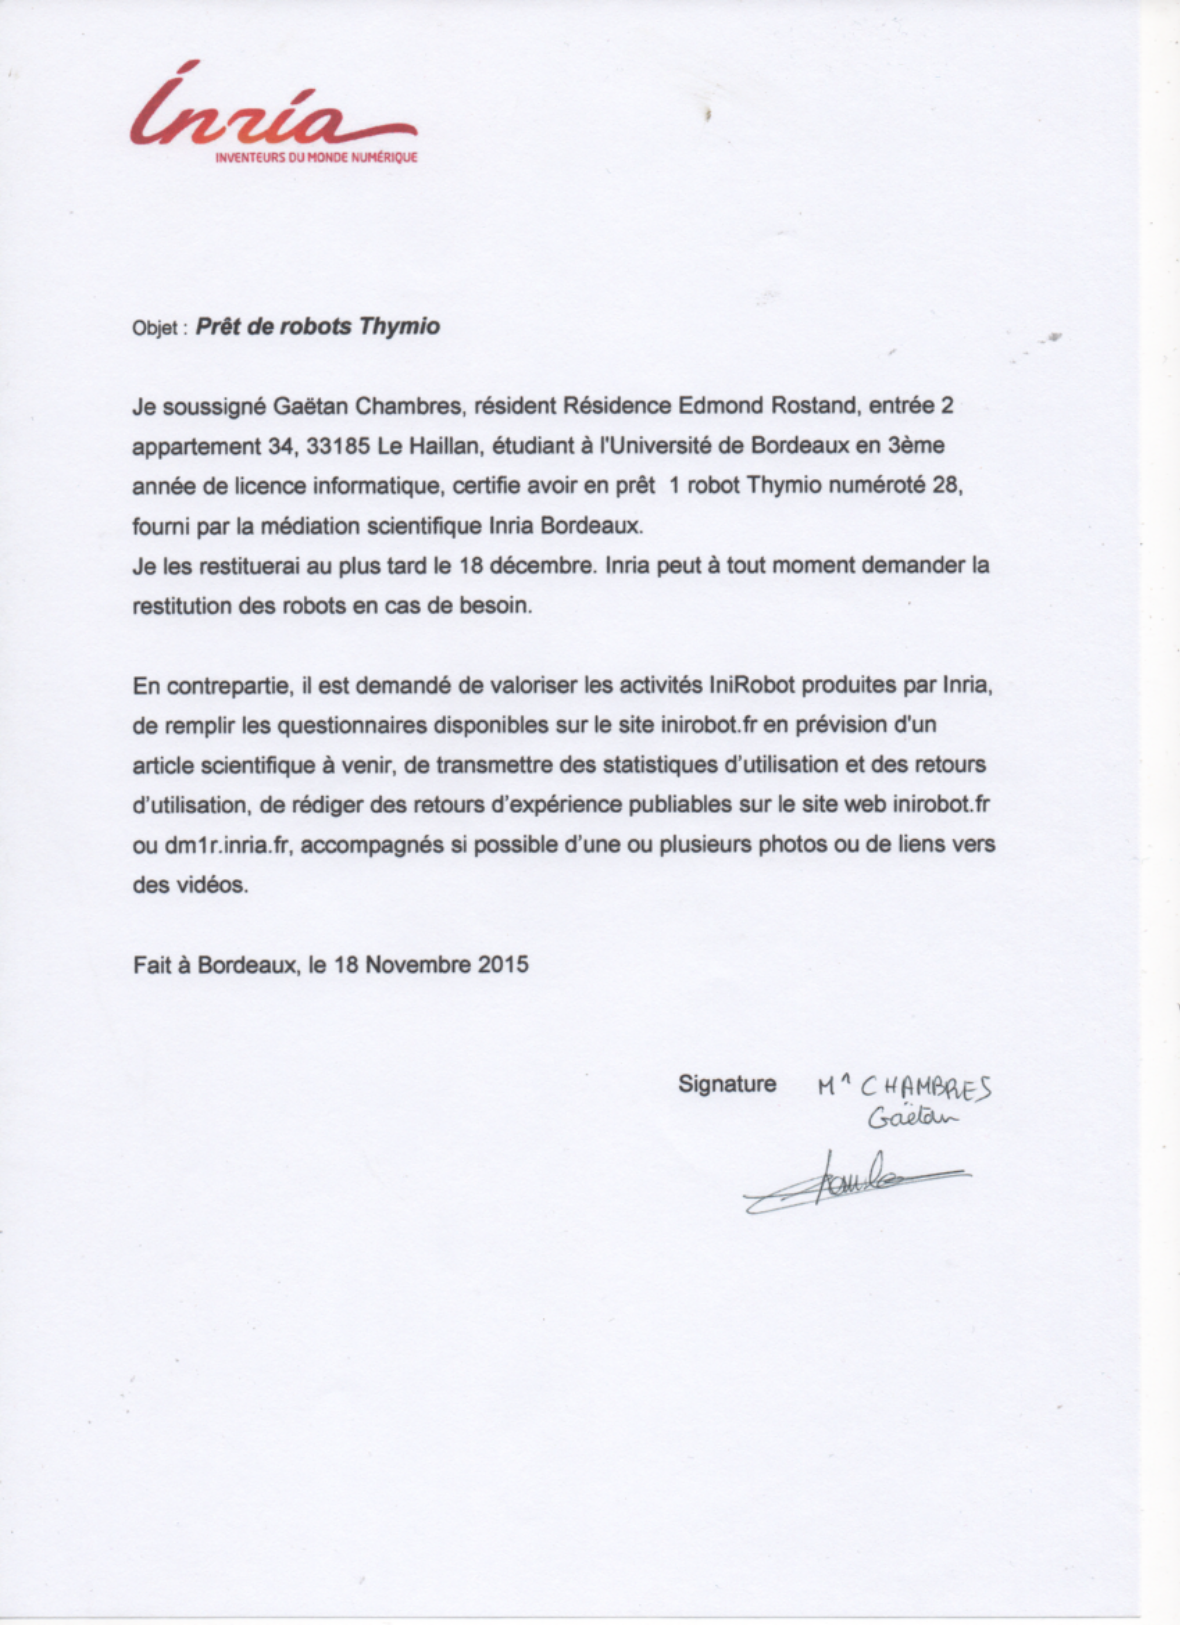
\includegraphics[width=0.9\textwidth]{pret.png}

\end{document}
